\chapter{Modello delle specifiche}
	\label{cap:modellospecifiche}

\section{Architettura}
La struttura associata all'Architettura da implementare può essere rappresentata semplicemente come in figura \ref{fig:architettura}
\begin{figure}[H]
	\centering
	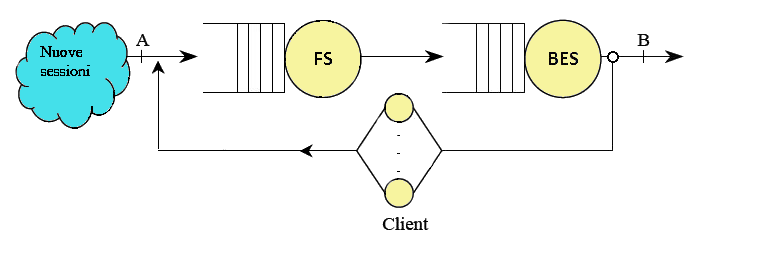
\includegraphics[scale=0.7]{img/architettura.png}
	\caption[Architettura del sistema]{Rappresentazione grafica dell'architettura del sistema.}
	\label{fig:architettura}
	\end{figure}
All’inizio della simulazione il primo evento che si verifica è sempre l'arrivo di una nuova sessione (evento NewSession).

\vspace{0.5cm}I client del centro nel ramo di retroazione sono paralleli ed infiniti.

\vspace{0.5cm}Ovviamente i nuovi eventi in arrivo verso il sistema verranno posti in coda al FrontServer, nel caso in cui non possano essere serviti. Come è possibile notare nella figura precedente, la sessione una volta servita dal Front Server verrà posta in coda verso il Back-End Server finché non verrà servita da quest'ultimo. Infine le sessioni saranno completate oppure poste nella zona di "\textit{Thinking}" finché non verranno reinserite nella coda del Front-End in attesa di essere serviti, passando attraverso un ramo di feedback.
 
\section{Clock di simulazione e schedulazione di  Eventi}
Nella fase implementativa si tiene conto dell'avanzamento del tempo per mezzo della variabile \textit{current\_time}. Il meccanismo di avanzamento del tempo scelto è il \textit{Next-Event Time Advance}. Questa scelta garantisce che gli eventi occorrano nella sequenza corretta. Si utilizza, inoltre, il flag di \textit{arrivals} per regolare l'accettazione delle nuove sessioni: se impostata a zero vengono inibiti i nuovi arrivi\footnote{Ovvero viene eseguito il drop della sessione in entrata o l'abort se la sessione è già nel sistema}, viceversa si procede normalmente con la simulazione.

\section{Event List}
Per la gestione degli eventi si utilizza una lista collegata di strutture \textit{Event}, come quella mostrata in figura, salvate in ordine crescente rispetto al tempo. Ogni nodo contiene il tempo di occorrenza e la sua tipologia. Un gestore di eventi è utilizzato per il demultiplexing di tale lista facendo uso di una funzione pop() per ottenere il \textit{Next-Event} da processare.
\begin{figure}[H]
  \centering
  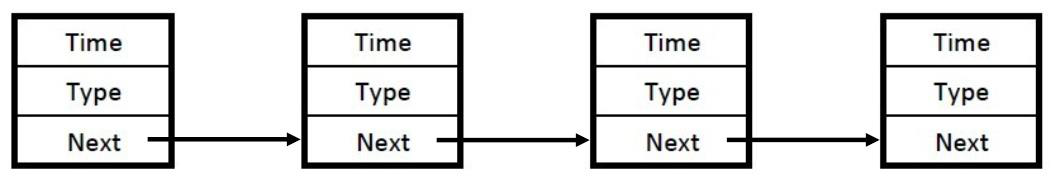
\includegraphics[scale=0.5]{img/EventList.png}
  \caption[EventList]{Struttura lista eventi}
  \label{fig:eventList}
\end{figure}

\section{Arrival Queue}
Al fine di ottenere informazioni riguardo i tempi di residenza che le sessioni sperimentano durante la loro permanenza nel sistema, si utilizzano delle strutture dati atte a registrare tali informazioni e ad usarle negli algoritmi del calcolo delle medie. Tali strutture, denominate \textit{ArrivalQueue}, immagazzinano i tempi di arrivo delle sessioni nelle sottosezioni del sistema (ovvero quando una sessione entra nel \textit{Front Server} o nella sua coda, quando entra nel \textit{Back-End Server}, e così via). Ad ogni completamento sperimentato da una sessione viene utilizzata la coda relativa e si calcola, per differenza, il tempo effettivo che la sessione ha passato in quella parte di sistema. Tutto ciò è possibile grazie all'ipotesi che l'ordine di arrivo, all'interno delle code del sistema, è sempre \texttt{preservato} la prima sessione ad entrare nella coda del Front Server, ad esempio, sarà la prima a lasciarlo.

\section{Request Queue}
Dal momento che è impossibile identificare una singola richiesta utilizzando la Next-Event Simulation, il problema di preservare l'informazione riguardante il numero di richieste attive di cui si compone una sessione viene risolto con la struttura dati \textit{Request Queue}. 

Ad ogni richiesta completata si decrementa il contatore delle richieste relative a quella sessione in modo da propagare tale informazione a tutte le richieste future. Quando il contatore arriva a zero la sessione viene completata del tutto e lascia il sistema.

\section{Client Order List}
Per preservare una Next-Event Simulation priva di contaminazioni derivanti da una possibile aggiunta di dati identificati delle sessione o delle richieste all'interno degli eventi di base, la Client Order List permette di conservare le informazioni relative all'ordine di arrivo e di uscita  degli utenti all'interno del centro Client. Attraverso questa informazione è possibile gestire il corretto ordine degli elementi della Request Queue nonostante siano condizionati da una mancanza di determinismo circa l'ordine di completamento degli utenti durante il loro periodo di Think Time.


\section{Personalizzazione del modello}
In base alle scelte effettuate dall'utente nella fase di \textit{setup} è possibile decidere di avviare la simulazione:
\begin{itemize}
\item senza \textbf{Overload Management}
\item con \textbf{Overload Management}
\end{itemize}
 
\noindent È possibile scegliere quale distribuzione utilizzare tra:
\begin{itemize}
\item \textit{Esponenziale}
\item \textit{10-Erlang}
\item \textit{Iperesponenziale}
\end{itemize}

\noindent \'E poi possibile impostare i parametri riguardanti lo \textit{STOP iniziale, STOP finale e Numero di Run}. Questi parametri sono utilizzati al fine di calcolare il passo\footnote{Per ``passo'' si intende l'incremento unitario dell'istante conclusivo di simulazione durante un insieme di run, nel calcolo del comportamento \textit{steady-state}} di ogni esecuzione mediante la seguente formula:

\begin{center}
 $Step = \frac{Stop Iniziale - Stop Finale}{Numero di Run}$
\end{center}

Giunta una nuova sessione, le richieste vengono accodate nel \textit{Front Server} in attesa di essere processate; effettuato il servizio, ovvero verificatosi un evento \textit{FS\_COMPLETION}, tale richiesta passa successivamente al servizio del \textit{Back-End Server}, al termine del quale si verifica un'occorrenza del tipo \textit{BES\_COMPLETION}. 

A questo punto il simulatore valuta per la suddetta sessione il numero di richieste rimanenti e effettua una scelta: se il numero di richieste di quella sessione è zero allora l'utente esce dal sistema; se, al contrario, così non fosse quest'ultimo attraverserà il ramo di feedback per esaurire le proprie richieste rimanenti.

%%Diagrammi per spiegazioni

\section{Avvio e fine simulazione}
Come unico vincolo per il termine della simulazione sono utilizzate due variabili, \textit{START} e \textit{STOP}, che regolano gli orari di apertura e chiusura del sistema.

\noindent Quest'ultimo inizia a schedulare eventi di tipo \textit{NewSession} solo dopo il tempo di \textsc{START} e inibisce tali eventi all'occorrenza del tempo di \textsc{STOP finale}.
\section{Algoritmi di Gestioni eventi}
\subsection{NewSession}
\begin{figure}[H]
  \centering
  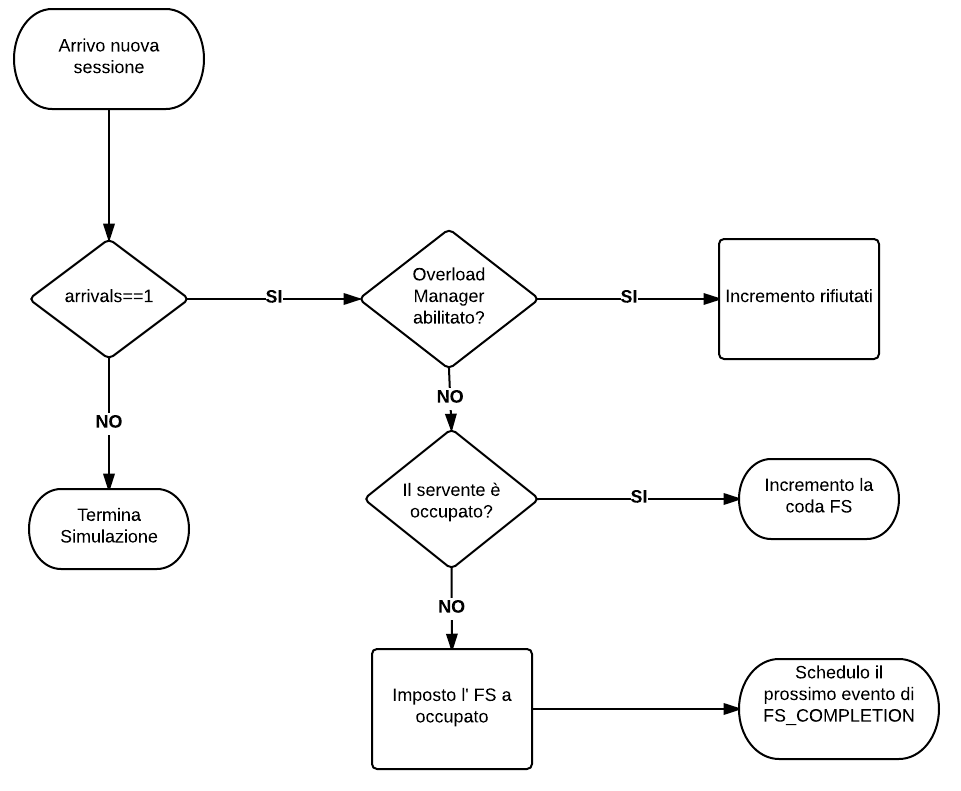
\includegraphics[scale=0.35]{img/NewSession.png}
  %\caption[NewSession]{Struttura lista eventi}
  \label{fig:NewSession}
\end{figure}
\subsection{FS Completion}
\begin{figure}[H]
  \centering
  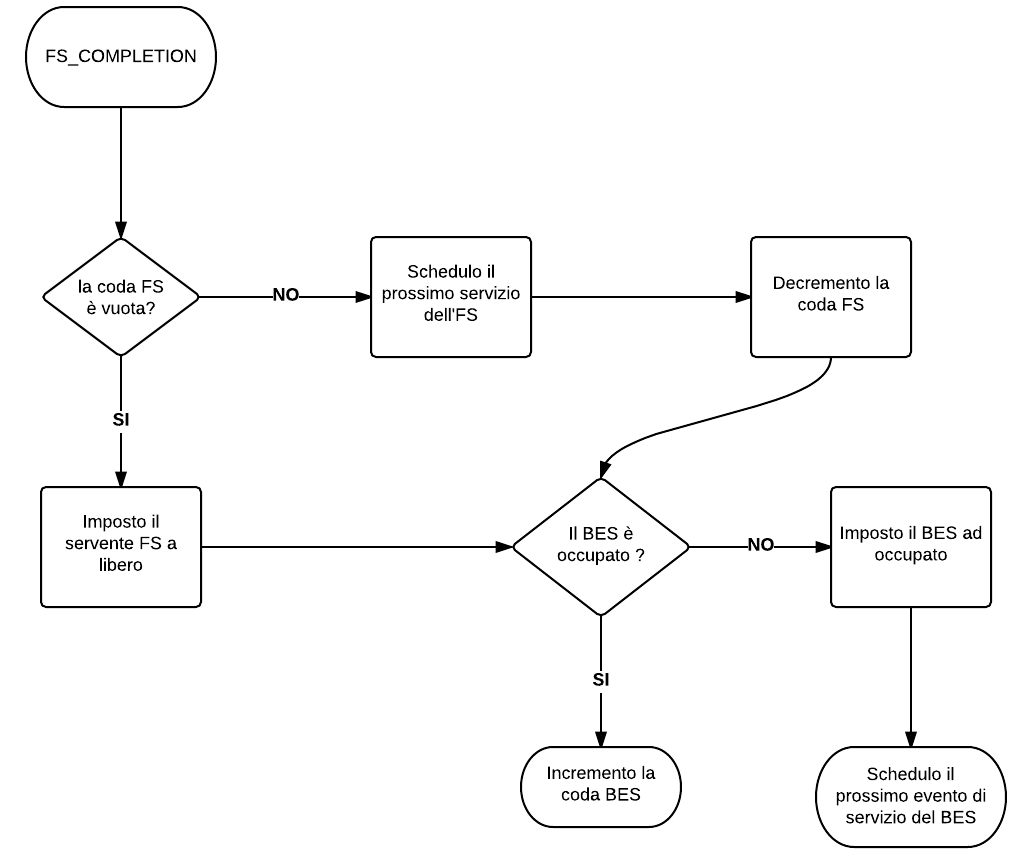
\includegraphics[scale=0.35]{img/FS_Completion.png}
  %\caption[NewSession]{Struttura lista eventi}
  \label{fig:FS_Completion}
\end{figure}

\subsection{BES Completion}
\begin{figure}[H]
  \centering
  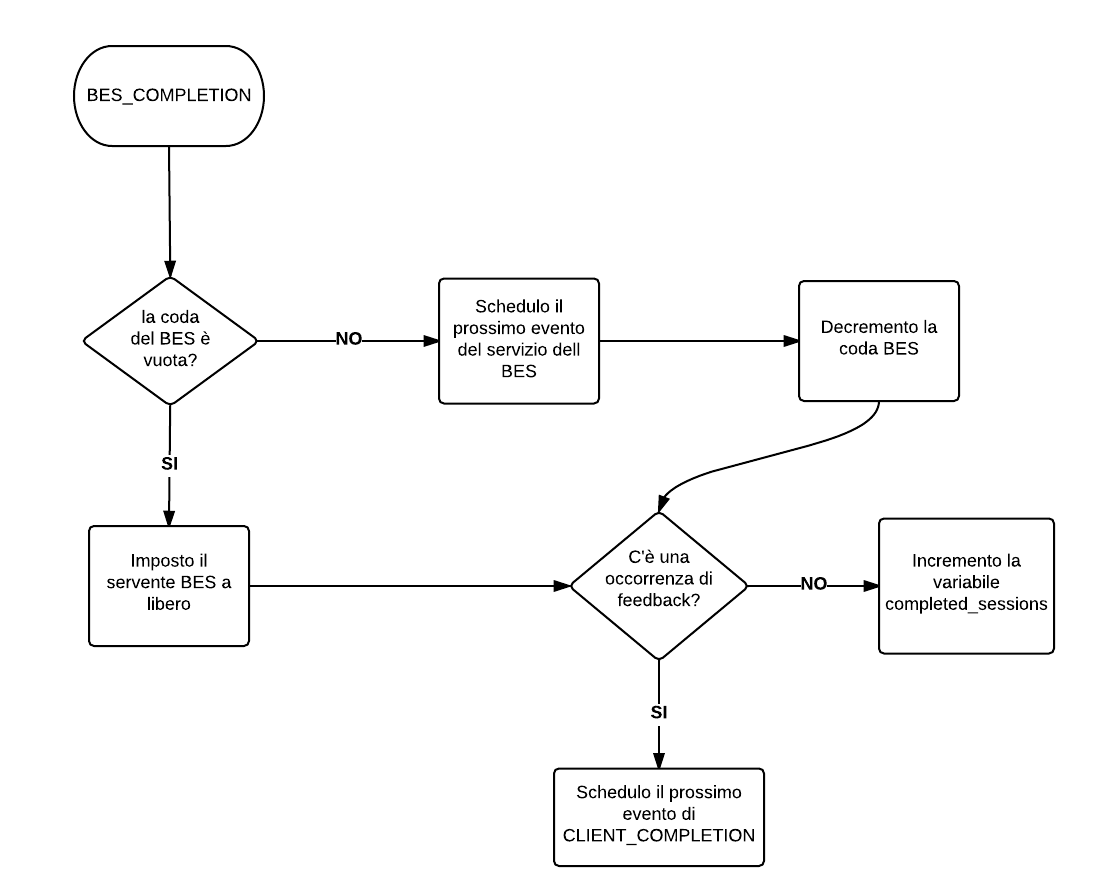
\includegraphics[scale=0.40]{img/BES_Completion.png}
  %\caption[NewSession]{Struttura lista eventi}
  \label{fig:FS_Completion}
\end{figure}

\subsection{Client Completion}
\begin{figure}[H]
  \centering
  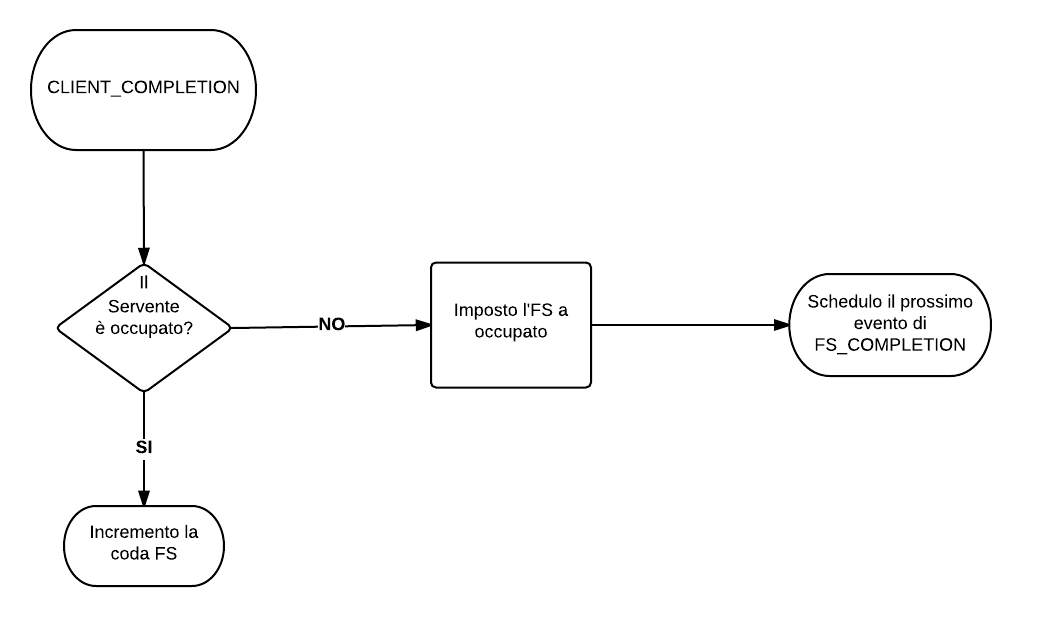
\includegraphics[scale=0.45]{img/CLIENT_Completion.png}
  %\caption[NewSession]{Struttura lista eventi}
  \label{fig:FS_Completion}
\end{figure}
\section{Dati esaminati}
Le richieste progettuali hanno sancito la raccolta di alcuni dati definite da alcune \textit{metriche} quali:
\begin{itemize}
\item \textbf{Troughput}:
è l'indice  che misura il totale di sessioni completate nell'unità di tempo. Tale indice viene calcolato attraverso il rapporto tra le sessioni totali processate dal sistema e l'intervallo di tempo necessario per ultimare questo compito.  Il troughput basato sulle sessioni è un ottimo indice per valutare il numero di utenti serviti dal sistema in un intervallo dato risultando una misura sensibile per l'utente finale. Per tener conto della capacità computazionale del sistema data dal numero di singole richieste completate , si è deciso di calcolare anche il troughput basato sulle richieste  attraverso un semplice rapporto tra il totale delle richieste processate dal sistema e l'intervallo di tempo utilizzato nell'eseguirle.

\item \textbf{Drop Ratio}:
misura il rapporto tra il totale delle sessioni rifiutate dal sistema ed il numero di sessioni totali che tentano di entrare nel sistema (accettate + rifiutate).

\item \textbf{Abort Ratio}:
è il rapporto tra le richieste abortite ed il totale di richieste processate dal sistema.
Questo è dovuto dal fatto che una richiesta può rientrare nel sistema, tuttavia in condizioni di saturazione, tale richiesta non è in grado di poter rientrare all'interno del Front Server, quindi viene appunto abortita.

\item \textbf{Tempo di Risposta del Sistema}:
viene inteso come la somma del tempo di risposta (Tempo in coda + Tempo di Servizio) del front-end e del back-end.
In pratica il tempo di risposta è inteso come il tempo che intercorre tra l'uscita di una richiesta dal centro di Client, ovvero la fine del periodo di "\textit{Thinking}" di un dato utente, ed il ritorno di tale richiesta al centro.



\end{itemize}
\begin{comment}
\section{Gestione degli eventi}
Vengono riportati nelle figure~\ref{fig:nuovasessione}~\ref{fig:completamentoFE}~\ref{fig:completamentoBE}~\ref{fig:completamentoT} i flussi di esecuzione di ogni evento:
\begin{center}	
	\begin{figure}[H]
	\centering
%	\includegraphics[scale=0.7]{Immagini/arrivo.png}
	\caption[Nuova Sessione]{Nuova Sessione}
	\label{fig:nuovasessione}
	\end{figure}
\end{center}

\begin{center}	
	\begin{figure}[H]
	\centering
%	\includegraphics[scale=0.7]{Immagini/compl_front-end.png}
	\caption[Completamento Front-End]{Completamento Front-End}
	\label{fig:completamentoFE}
	\end{figure}
\end{center}

\begin{center}	
	\begin{figure}[H]
	\centering
%	\includegraphics[scale=0.7]{Immagini/compl_back-end.png}
	\caption[Completamento Back-End]{Completamento Back-End}
	\label{fig:completamentoBE}
	\end{figure}
\end{center}

\begin{center}	
	\begin{figure}[H]
	\centering
%	\includegraphics[scale=0.7]{Immagini/compl_think.png}
	\caption[Completamento Think]{Completamento Think}
	\label{fig:completamentoT}
	\end{figure}
\end{center}
\end{comment}
\begin{comment}
\section{Metriche}
Nella traccia viene richiesto di calcolare le seguenti quattro metriche:
\begin{itemize}
\item Il \textbf{Throughput} è l'indice di prestazione che misura il totale di sessioni completate per unità
di tempo. Tale indice viene calcolato attraverso il rapporto tra le sessioni totali e l'intervallo di tempo necessario per il processamento.
\item Il\textbf{Dropped Ratio} misura il rapporto tra il totale delle sessioni rifiutate dal sistema ed il numero di sessioni totali che tentano di entrare nel sistema (accettate + rifiutate).
\item L'\textbf{Aborted Ratio} è il rapporto tra le richieste abortite ed il totale di richieste processate dal sistema
\item Il \textbf{Tempo di Risposta del sistema} inteso come somma del tempo di risposta\footnote{Tempo in coda più tempo di servizio} del front-end e del back-end.
\end{itemize}
\end{comment}

\section{Modello Analitico}
Al fine di prevedere, in linea di massima, i risultati del simulatore, viene elaborato un modello  analitico semplificato per poter studiare il sistema preso in esame.
Il sistema implementato presenta numerosi vincoli ed una complessità insita nelle specifiche, a tal proposito viene proposto un modello volontariamente e lievemente differente dal caso reale, fornendo un limite inferiore delle prestazioni e degli indici misurati.

Il sistema esaminato risulta essere interattivo, in quanto avviene uno scambio di richieste tra Client e Server, con un comportamento a rete aperta ( le nuove sessioni possono entrare nel sistema qualora questo non fosse saturo), a tal proposito si è deciso di presentare due modelli differenti tra loro, uno a rete aperta ed uno a rete chiusa. Questi permettono di descrivere in dettaglio la maggior parte degli elementi che costituiscono il sistema stesso.

\section{Modello semplificato a rete aperta}
In questo primo modello si ha una rete aperta di Jackson con un tasso di sessioni in
arrivo pari a $\gamma$ . Si è deciso così, per questioni di semplificazione del modello, di non
inserire, come componenti, la Priority Queue e il centro di client, in quanto
risultavano di difficile analisi in un modello di rete aperta come quello di Jackson.
\begin{center}	
	\begin{figure}[H]
	\centering
	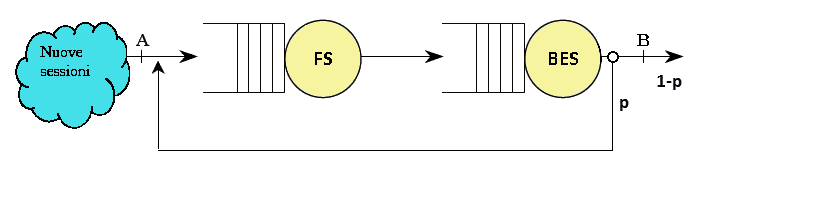
\includegraphics[scale=0.7]{img/reteJackson.png}
	\caption[Modello a rete aperta]{Modello a rete aperta}
	\label{fig:Modello a rete aperta}
	\end{figure}
\end{center}

$\gamma = 35 sessioni/s$

$\vspace{2mm}$

$\begin{cases} 
\lambda_{1} = \gamma + p \lambda_{2} \\ \lambda_{2} = \lambda_{1} \\
\end{cases}$  $\rightarrow$
$\begin{cases} 
\lambda_{1}(1-p) = \gamma \\ \lambda_{2} = \lambda_{1} \\
\end{cases}$ $\rightarrow$
$\begin{cases} 
\lambda_{1} =\frac{ \gamma}{(1- p)} \\ \lambda_{2} =\frac{\lambda_{2}}{(1-p)} \\
\end{cases}$
$\vspace{2mm}$
$\lambda_{1} = \lambda_{2} = \frac{\gamma}{(1-p)} ; p=\frac{19}{20} \rightarrow \lambda_{1} = \lambda_{2} = 35\times20 = 700 richieste/s$
$\vspace{2mm}$

$\lambda_{1}\gg\mu_{FS}; \lambda_{2}=\mu_{FS} poiché \mu_{BES}\gg\lambda_{1}$
$\vspace{2mm}$
Viene quindi calcolato il throughput, ovvero il numero di sessioni che escono dal sistema al secondo:
$\vspace{2mm}$

$\lambda_{2} =\frac{\lambda_{2}}{(1-p)}=\frac{\mu_{FS}}{20}\approx\frac{219}{20} richieste/s =X_{sessioni}$
$\vspace{2mm}$
$\vspace{2mm}$
$X_{richieste}=X_{sessioni}\times20$
$\vspace{2mm}$
Per quanto concerne l'indice riguardante la percentuale di sessioni rifiutate dal sistema, si trova:
$\vspace{2mm}$

$dropped=\frac{\#sessioni accettate}{\#totale arrivi}$ $\rightarrow$ $\frac{35-X_{sessioni}}{35} = 1-\frac{2}{7}\approx 0.7$ $\rightarrow$ $\%dropped \approx 70\%$

\section{Modello semplificato chiuso}
\begin{center}	
	\begin{figure}[H]
	\centering
	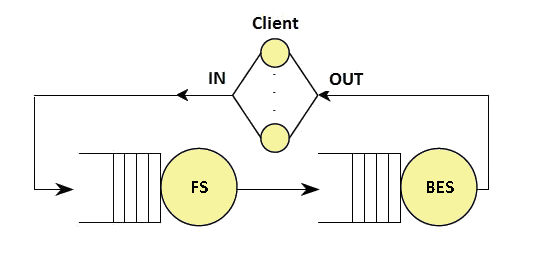
\includegraphics[scale=0.7]{img/retechiusa.png}
	\caption[Modello a rete chiusa]{Modello a rete chiusa}
	\label{fig:Modello a rete aperta}
	\end{figure}
\end{center}

$D_{FS}=0.00456; D_{BES}=0.00117; E[Z]=7s ; N=250$ (in realt\'a il numero aumenta costantemente!)
$\vspace{2cm}\hspace{2mm}$
$\vspace{2mm}\hspace{2mm}$Anche qui si può calcolare il throughput del sistema, come:
$\vspace{2mm}$
$X = min\{\frac{1}{D_{max}},\frac{N}{D+Z}\}= min\{\frac{1}{D_{FS}},\frac{250}{D_{FS}+D_{BES}+Z}\}=35.685 richieste/s$
$\vspace{2mm}$
Da cui si pu\'o ricavare il lower bound per il tempo medio di risposta.
$\vspace{2mm}$
$E[R]\geq max\{D,\frac{N}{X}-E[Z]\}= max \{0.00573,\frac{250}{35}-7\}\approx0.0057447$

